\documentclass{beamer}

\usepackage{graphicx}
\usetheme{Szeged}
\usecolortheme{beaver}

\author{Anne Wanningen \and Xeryus Stokkel}
\title[Week 2]{Introduction to Computer Graphics OpenGL week 2}

\begin{document}

\maketitle

\section{Control modes}
\begin{frame}
	\begin{itemize}
		\item Click \& drag
		\item Just drag
		\item FPS 'no-clip' mode
	\end{itemize}
\end{frame}

\section{Screenshots}
\begin{frame}
	\begin{figure}
		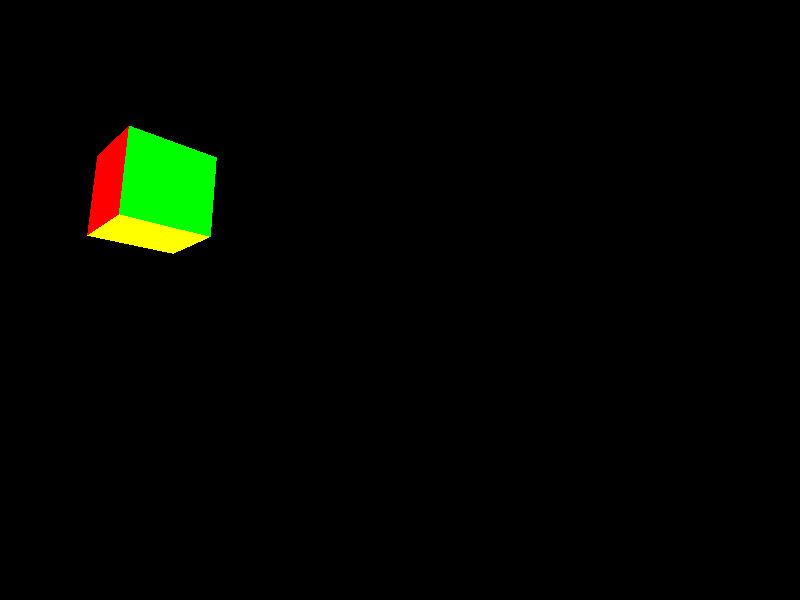
\includegraphics[height=.8\textheight]{oglcubefps.png}
	\end{figure}
\end{frame}

\begin{frame}
	\begin{figure}
		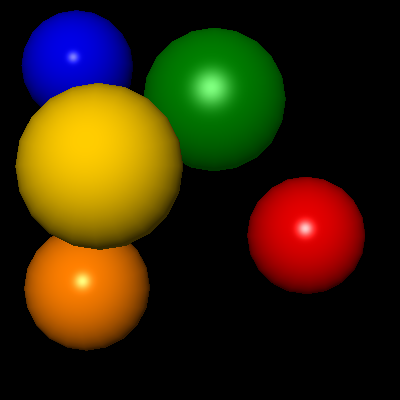
\includegraphics[height=.8\textheight]{oglscene01.png}
	\end{figure}
\end{frame}

\begin{frame}
	\begin{figure}
		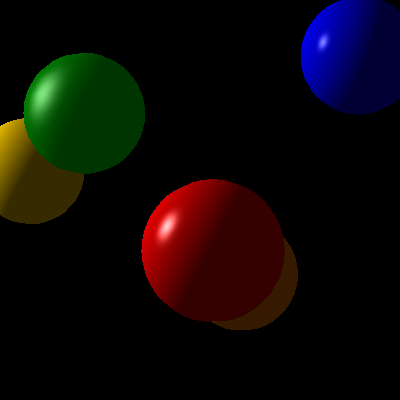
\includegraphics[height=.8\textheight]{oglrot1.png}
	\end{figure}
\end{frame}

\end{document}